\chapter{The Level 1 trigger upgrade} % 
\label{sec:triggerUpgrade}

During Run 2, the LHC has provided collisions at energy of 13\TeV~and at up 
to a peak luminosity of $14\times10^{33}cm^{-2}s^{-1}$, marking a signifcant increase
in peak energy and luminosity provided during Run 1 (8\TeV~and $7\times10^{33}cm^{-2}s^{-1}$).
At 25ns bunch spacing an average of 25 simlutaneous interactions are produced.
The instantaneous luminosity and pileup provide a challenging environment for the L1 trigger system
during Run 2, exceeding design specifications. The rate into the HLT must 
remain at 100kHz. Simply increasing thresholds on the L1 trigger seeds would imply
unacceptable inefficiencies for electroweak physics and \TeV~ scale searches
at CMS and so the L1 trigger system, and associated algorithms, must be upgraded. 

In the following, the upgrades to the L1 calorimetric trigger system and the 
associated L1 jet algorithm are discussed. The muon trigger system 
and upgrades to the algorithms for identification of other physics objects for the L1 trigger are discussed 
in~\cite{ele_algo,tau_algo,muon_algo}.


\section{Legacy system and upgrade}

The Global Calorimeter Trigger (GCT) was used during Run 1 to find jets, electrons and photons and to 
compute global energy sums \cite{gct}. The trigger system takes input from trigger towers (TT) corresponding to $5\times5$ ECAL crystals 
and an identical area in the HCAL. These are grouped into $4\times4$ \emph{regions} which form the input for physics object and
reconstruction algorithms. These inputs are provided by Trigger Primitive Generators (TPGs). 
Due to hardware limitations the detector is split into 16 
regions which are processed by separate Regional Calorimetric Triggers (RCTs) to form candidates and sum 
energies. The RCTs must share information to account for features which occur at boundaries between 
them. The information from the RCTs is combined in the GCT which computes global quantities and sorts 
the jets before sending to the Global Trigger which also receives the Muon trigger
information and makes the final trigger decision. 

The upgrade of the GCT was carried out in two stages. The first stage
Upgrade Calorimetric Trigger (UCT) was used for data taking during 2015
and used updated firmware and algorithms to allow improved pileup subtraction 
and improved jet and object identification \cite{uct}. In the second stage the 
architecture was entirely replaced to allow \emph{time multiplexing} (TMT) whereby each
event is processed entirely within one card using the full trigger tower granularity. 

\subsection{Stage 2 Calorimetric trigger upgrade}

The Stage 2 calorimetric trigger uses two processing layers. The first, layer 1, performs
pre-processing and data formatting using 18 CTP7 cards \cite{}. Each card requires
only a regional view of the detector and performs local operations such as summing 
ECAL and HCAL transverse energies. The data for each event is combined and transmitted to 
a single node in the layer 2, an Imperial Master Processor Virtex-7 (MP7) card. 
The MP7 is a high performance 0.92Tb/s + 0.92Tb/s (input + output rate) all-optical processor \cite{mp7}
with sufficient data rate for the entire calorimeter to be processed in a single card. The data 
from the 9 layer 2 nodes is sent to a demultiplexer board (also an MP7) to be formated before
the data is sent to the Global Trigger.

The difference between the GCT and TMT architectures is shown in Figure~\ref{tmux}. 
In the TMT architecture, data is buffered and retransmitted to the first node (on layer 2)
over 9 bunch crossings to allow the entire event to be processed on one card. This
removes the need for a large number of links between cards and allows the full trigger
tower granularity to be used. The increase in granularity compared to the GCT is
illustrated in Figure~\ref{fig:inputres}. 

\begin{figure}

\centering
    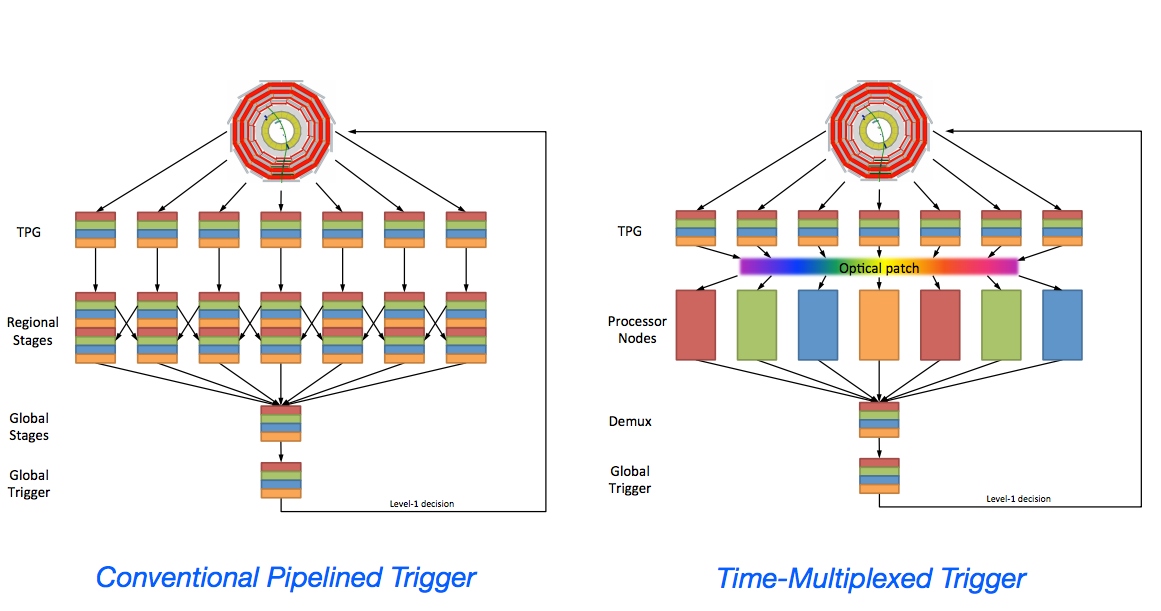
\includegraphics[width=0.9\textwidth]{./Figures/triggerUpgrade/tmux}
  \caption{Comparison of the GCT (left) and TMT architectures (right) showing the flow of information
  to the final global decision. The colours indicate the data from each bunch crossing. \cite{tmt}}
  \label{tmux}
\end{figure}

\begin{figure}
\centering
\subfigure[Input resolution: GCT]{
\includegraphics[width=0.35\textwidth]{./Figures/triggerUpgrade/L1inputreslegacy.png}\label{subfig:inputlegacy}} \quad
\subfigure[Input resolution: stage 2 upgrade]{
\includegraphics[width=0.35\textwidth]{./Figures/triggerUpgrade/L1inputresupgrade.png}\label{subfig:inputupgrade}} 
\caption{A representation of the CMS collaboration logo digitised with the input resolution of the L1 calorimeter trigger up to 
\etaabs~$< 3$ using (a) the legacy system ($18 \times 14$ pixels) and (b) the stage 2 upgrade ($72 \times 56$ pixels).}
\label{fig:inputres}
\end{figure}

\section{Level-1 jet algorithm upgrade}
\label{algo}

The increase in pileup and luminosity in Run 2 makes triggering with jets
significantly more challenging than during Run 1. To maintain sensitivity to
new physics the new algorithm must allow high efficiencies and
low rates even for high pileup scenarios.

The stage 2 upgrade provides several advantages over the GCT system which can be 
exploited in designing the jet algorithm, including significantly increased processing power
and granularity (enhanced by factor 16). This allows more flexible algorithms, which can 
exploit smaller features than previously accessible, to be defined. This is exploited in the 
use of an improved jet clustering (described in Section\ref{sec:jet_algo}) algorithm as well as 
online pileup subtraction techniques (described in Section ??) in the upgrade jet 
identification and reconstruction algorithm.

\subsection{Level-1 jet clustering}
\label{sec:jet_algo}
The GCT algorithm uses a $3\times3$ calorimeter region sliding jet window with a central seed 
to reconstruction jets in the range $|\eta| < 5$. The algorithm scans the calorimeter in increments
of regions and clusters a jet if the energy in the central seed region is greater than 
both $5\GeV$ and each of the eight bordering regions. The threshold of $5\GeV$ was added during 
the 2012 8\TeV run, when the number of pileup interactions increased, to remove soft pileup jets.
The $12\times12$ TT ($\Delta\eta\times\Delta\phi = 1.04\times1.04$) jet size corresponds 
approximately to $R=0.5$ for the anti$k_T$ jet algorithm used in offline reconstruction.

The jet algorithm used for the stage 2 upgrade similarly uses a sliding window algorithm. This
is composed of $9\times9$ TTs ($\Delta\eta\times\Delta\phi = 0.78\times0.78$), corresponding 
to the $R=0.4$ used in Run 2. The use of an odd number of trigger towers ensures a central 
seed tower can be defined. In designing the algorithm various central seed thresholds have 
been considered, as discussed below.

In order to ensure that jets do not overlap the seed tower is required to meet the conditions
shown in Figure~\ref{mask}. The veto conditions are asymmetric along the diagonal to ensure  
that TTs with the same energy cannot veto one another. These veto conditions ensure that there 
is no double counting of overlapping jets. An inefficiency may be expected 
as one jet may veto another which itself vetoes a third. However, this effect was found to 
introduce a negligible (~0.1\%) inefficiency.

If a seed passes the veto requirements a jet is defined with a position given
by the seed position and an energy given by the total energy of the towers. The position is
given by that of the seed as jets tend to be boosted objects with an energy deposited in
a small central area.

\begin{figure}
\centering
    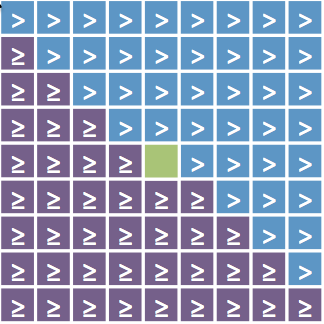
\includegraphics[width=0.5\textwidth]{./Figures/triggerUpgrade/mask.png}
  \caption{The $9\times9$ veto conditions used to define jets. The inequalities ensure
  jet energies are not double counted}
  \label{mask}
\end{figure}

\section{Pileup Subtraction}
\subsection{Pileup}

The luminosity of the LHC will be increased in the upgrade to a maximum of 
$L = 1.4\times10^{34} cm^{-2}s^{-1}$. The easiest way to increase luminosity while maintaining stability is to 
use large, but widely separated, proton bunches \cite{PUform}. However, for the detector this means increased 
number of primary vertices (pileup) at the collision point. The average number of interactions per 
bunch crossing is given in equation \ref{pu}.

\begin{equation}
\langle N_p \rangle = \sigma L 
\tau_b
\label{pu}
\end{equation}

where $\langle N_p \rangle$ is the average number of interactions, $\sigma$ 
is the cross section and $\tau_b$ is the bunch spacing. At the end of run 
1 with $8 TeV$ ($\sigma = 71.5mb$), $\tau_b = 50ns$ and $L = 0.75\times10^{34} cm^{-2}s^{-1}$ 
gave $\langle N_p \rangle\simeq27$. After LS1 the luminosity and $\sigma$ gain (to $76mb$) will increase 
this to $\langle N_p \rangle\simeq40$. 
\subsection{Effect of Pileup}
The majority of pileup events are low 
energy QCD processes which will appear as randomly distributed energy in the calorimeter region (about 
1 GeV per unit area). This pileup can have two detrimental effects for the L1 
trigger. Firstly, when the pileup is evenly distributing the energy of the real jets is 
slightly increased, thus artificially increasing the total transverse energy. The second problem occurs when the 
pileup is randomly clustered - significantly boosting a single jet or forming fake jets. Due 
to the imperfect response of the detector and profile of the pileup these effects may 
be dependent on $\eta$. In order to trigger only on hard events the effect of 
the pileup must be mitigated (subtracted). In this report two example methods of pileup subtraction 
(global $\rho$ and donut) will be discussed.
\subsection{Global $\boldsymbol{\rho}$}
If the detector response is assumed 
to be approximately $\eta$ independent then one may use an event based pileup subtraction. In 
the case of global $\rho$ first all the jets are reconstructed using the algorithm in 
\ref{algo}. The jets are then ranked in order of energy density $\rho$ where for jet 
$i$, $\rho^i$ is defined in equation \ref{rho}.
\begin{equation}
\label{rho}
\rho^i = \frac{p^i_{T}}{A_i} 
\end{equation}
where $A_i$ 
is the area of the jet. The median $\rho$ ($\rho^m$) of the jets is then 
taken as the estimator of the pileup energy density in the event \cite{jetarea}. All jets 
are in the event then reduced in energy by $\rho^m \times A^i$ and those with 
$p_{T}^i < \rho^m \times A_i$ taken to be pileup and removed. The correlation of this 
parameter with the number of interactions is shown in figure \ref{rhonint}. This method has the 
advantage of being stable against fluctuations, however, local effects are not considered and there is 
an inherent under-subtraction bias in the event as the pileup jet $p_{T}$ forms a bound 
on the energy subtracted per jet.
\subsection{Donut Subtraction}
\begin{figure}
\centering
    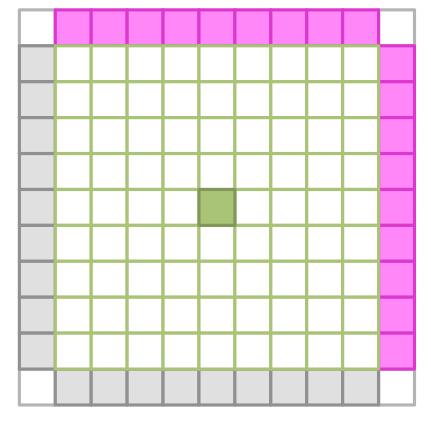
\includegraphics[width=0.5\textwidth]{./Figures/triggerUpgrade/donut}
  \caption{Donut ring for pileup 
  estimate. Neglecting the corners the pileup energy density is taken as that in the 
  middle two strips.}
  \label{mask}
\end{figure}  
Donut subtraction takes advantage of the area around each 
jet to make a local subtraction. The energy contribution from the jet is expected to 
be negligible by the outside ring ($\Delta R^2\simeq 0.2$) \cite{jetmet}. Taking the four strips around 
the jet as shown in figure \ref{donutnint} they are ordered in energy and the pile 
up energy density ($\rho_d$) is taken as the energy of the middle strips divided by 
their area ($A_d$). This energy density is then subtracted from the jet as for global 
$\rho$. The dependence of $\rho_d$ on number of vertices is shown in figure \ref{donutnint}. The 
highest strip is neglected to remove the contamination of nearby jets and the lowest to 
account for edge effects. Unlike global, donut subtraction allows local dependence of pile up to 
be taken into account, however, it is susceptible to fluctuations as the sampling region is 
small.

An additional method to remove pure pileup jets is to require a seed 
threshold. This takes advantage of the fact that pileup jets have flatter topologies. This is 
because, unlike the jets from the primary vertex, they are made from clusters of uniform 
pileup. A threshold on the seed tower can thus reduce the rate of pileup while 
maintaining efficiency. Donut subtraction may then be performed to correct the remaining jets. A seed 
threshold is not possible before the global $\rho$ calculation as this relies on lower $p_{T}$ 
jets for the pileup estimation. Optimising the seed (perhaps as a function of $\eta$) is 
under way, however, a threshold of 2.5GeV (5 level one units) was chosen as a 
benchmark.

\begin{figure}
\hfill
\subfigure[Global $\rho$ \label{rhonint}]{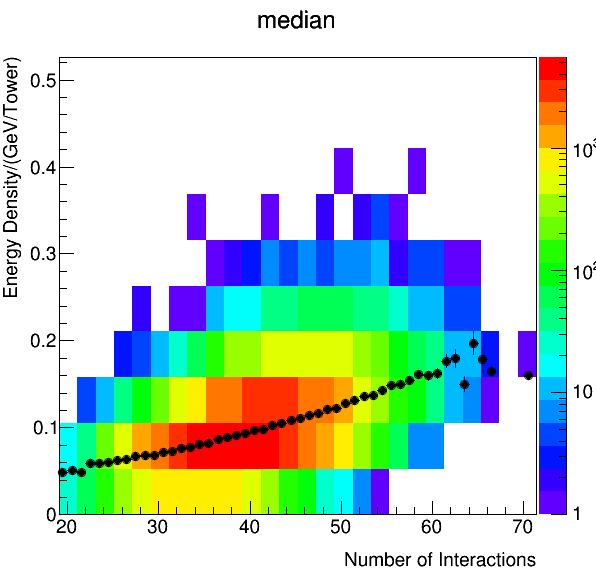
\includegraphics[width=7cm]{./Figures/triggerUpgrade/strips_median}}
\hfill
\subfigure[Donut Subtraction\label{donutnint}]{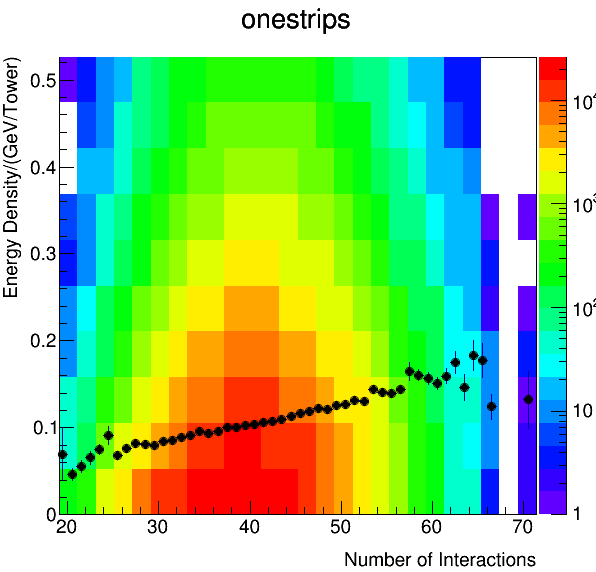
\includegraphics[width=7cm]{./Figures/triggerUpgrade/strips_onestrips}}
\hfill
\caption{Dependence on the number 
of interactions of the two pileup subtraction regimes studied.}
\end{figure}

\section{Jet Algorithm}
\subsection{Efficiencies}
In 
order to test the jet finding algorithm the first study that must be undertaken is 
into the matching efficiency of the L1 jets to generator level quantities (gen jets). A 
simulated sample of $t\bar{t}$ pairs was used\footnote{In this report all simulated samples used have conditions 
of $13TeV$ collisions with bunch spacing $50ns$. The pileup is gaussian distributed around $40$ interactions 
per bunch crossing}. The gen jets are made by running the anti-kt algorithm with radius 
parameter $R=0.4$ on generator level quantities. The gen jet is said to be matched if 
it is within ${\Delta R}^2<33$ of a L1 jet (the greatest extent of the L1 
jet). The matching efficiency for alljets and the fourth jet is shown in figure \ref{match}. 
It can be seen that the efficiency after pileup subtraction/seed drops at low $p_T$. This 
motivates a cut at $30GeV$ for the calculation of energy sums. Inefficiencies at high $p_T$ 
are caused by the `chain veto', however, the jet algorithm guarantees there is always a 
comparable or higher jet in the event in such cases. The performance compared to GCT 
is seen to be greatly improved.  
\begin{figure}
\hfill
\subfigure[All jets\label{fig:label:alljet}]{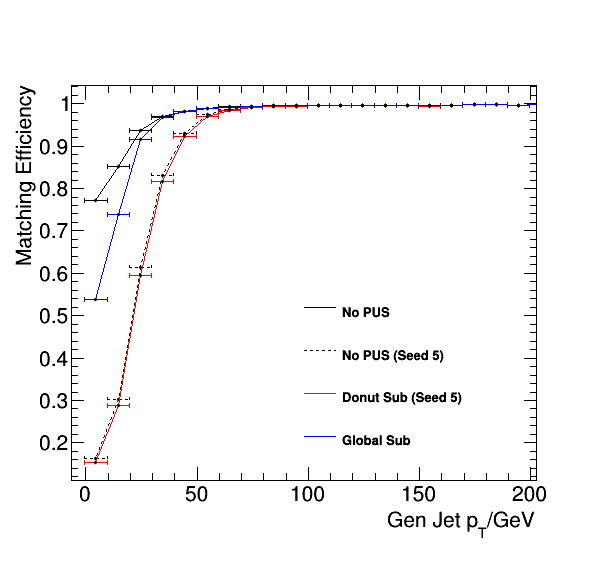
\includegraphics[width=6.9cm]{./Figures/triggerUpgrade/alljet}}
\hfill
\subfigure[4th jet\label{fig:label:jet4}]{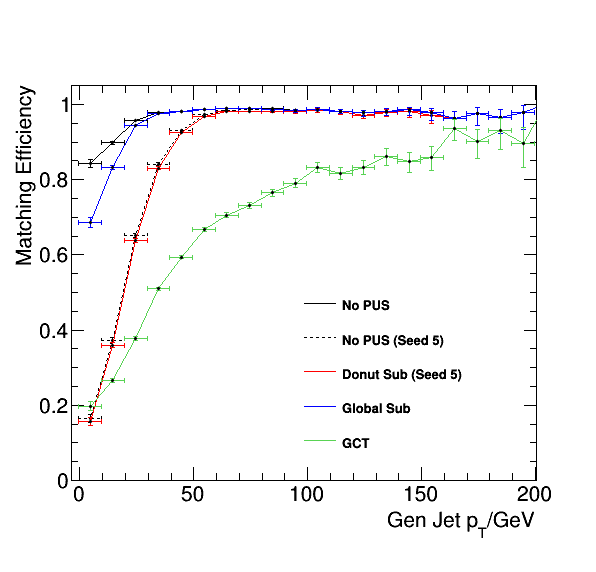
\includegraphics[width=7cm]{./Figures/triggerUpgrade/jet4}}
\hfill
\caption{Matching 
efficiencies for jets showing effect of seed and pileup subtraction at low energies. In \ref{fig:label:jet4} 
a comparison with the GCT is shown.}
\label{match}
\end{figure}
\subsection{Calibration}
The energy of the L1 
jets is calibrated using generator level quantities. The scheme for calibration is outlined in \cite{l1jet_calibration}. 
The calibration is carried out in bins of $\eta$ to account for the difference in 
performance of the detector. Using a QCD sample, the response (defined as $p^{L1}_{T}/p^{gen}_{T}$) and $p^{L1}_{T}$ 
are plotted against $p^{gen}_{T}$ and fitted. The fits are then plotted against each other and 
the result itself fitted. This gives calibration factors as a function of $p^{L1}_{T}$.  Where the 
matching efficiency is low it is not possible to fit and so the calibration has 
a lower bound on $p_T$. This was found to occur at $30GeV$. An upper bound 
is defined by where the fits become statistically limited. This was found to occur at 
$300GeV$. If the fit is well defined the calibration factor should flatten with increasing $p_T$ 
and so higher $p_T$ jets may still be calibrated by continuing the fit. The calibration 
factors change depending on the pileup subtraction regime. In figure \ref{calib} the effect of the 
calibration is shown.   

\begin{figure}
\centering
    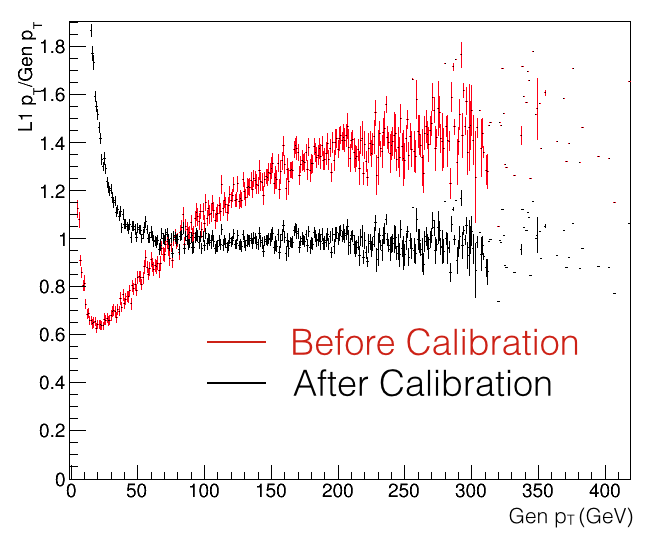
\includegraphics[width=7cm]{././Figures/triggerUpgrade/calibration}
  \caption{Effect of calibration on donut subtracted jets. At 
  the limit of calibration ($30GeV$) the difference for the calibrated sample is around $10\%$.}
  
  \label{calib}
\end{figure}
\section{Pileup Subtraction}

\subsection{Resolution Dependence on Number of Interactions}
In this section 
plots are shown for the highest $|\eta|$ bin as the detector performance is expected to 
worsen with larger $|\eta|$ and so pileup subtraction will have the largest effect. The first 
test of any pileup subtraction scheme is the effect on the resolution. In an ideal 
post pileup subtraction scenario this will be flat as a function of the number of 
interactions. In figure \ref{fig:label:resolution1} this is plotted for a particular $p^{gen}_T$ and $\eta$ bin. It 
can be seen that the response flattens for both pileup subtraction regimes. This is summarised 
in \ref{fig:label:resolution2} where the gradient from the fit to the resolution plot is shown to 
reduce after pileup subtraction for a range of $p^{gen}_T$ bins.  
\begin{figure}
\hfill
\subfigure[\label{fig:label:resolution1}]{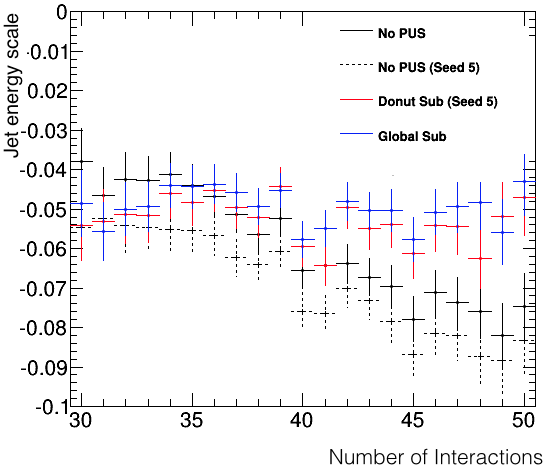
\includegraphics[width=6.8cm]{./Figures/triggerUpgrade/resolution}}
\hfill
\subfigure[\label{fig:label:resolution2}]{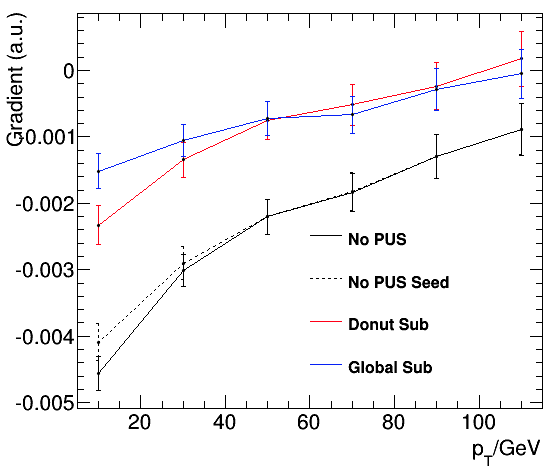
\includegraphics[width=7.1cm]{./Figures/triggerUpgrade/p1eta_14to28_calib_fits}}

\caption{In \ref{fig:label:resolution1} response versus number of interactions is shown for a particular eta bin showing 
the response flattens after pileup subtraction. In \ref{fig:label:resolution2} the fit gradient for different $p^{gen}_{T}$ bins 
is shown.}
\label{fig:label:resolution}
\end{figure}
\subsection{Rates and Efficiencies}
The rate is defined as the number of 
background events passing selection per second. The nominal rate for the L1 trigger is $\mathcal{O}100kHz$. 
The efficiency is then the proportion of signal events which trigger. To evaluate this a 
cut is made on the gen jets ($50GeV$). The proportion of these events with a 
corresponding matched L1 jet over a threshold then defines the efficiency at that threshold.  For 
the trigger, the key test is to see that the efficiency for signal may be 
maintained while reducing the background rate. For the background a pure pileup sample was used 
while the $t\bar{t}$ samples was used for signal. In figure \ref{fig:label:ratejet1} the rate is shown 
for the leading jet. The performance compared to the GCT is shown to be improved. 
The seed cut appears to have the largest effect in reducing the rate as global 
is shown to be comparable to no pileup subtraction. Figure \ref{fig:label:ratenvtx} shows the evolution of 
the rate with the number of interactions. GCT shows the largest dependence, as expected, while 
for stage 2 pileup subtraction is shown to decrease this dependence. Applying donut subtraction appears 
to increase the rate compared to applying a seed alone. This may be due to 
contamination causing over subtraction. The calibration will then bring the energy above the seed. Finally, 
in figure \ref{fig:label:rateeff} the rate is shown against efficiency for the lead jet. The seed 
is shown to be comparable to global subtraction alone while applying donut subtraction worsens the 
performance. This may again be due to contamination.
\begin{figure}
\hfill
\subfigure[Jet 4 Rate\label{fig:label:ratejet1}]{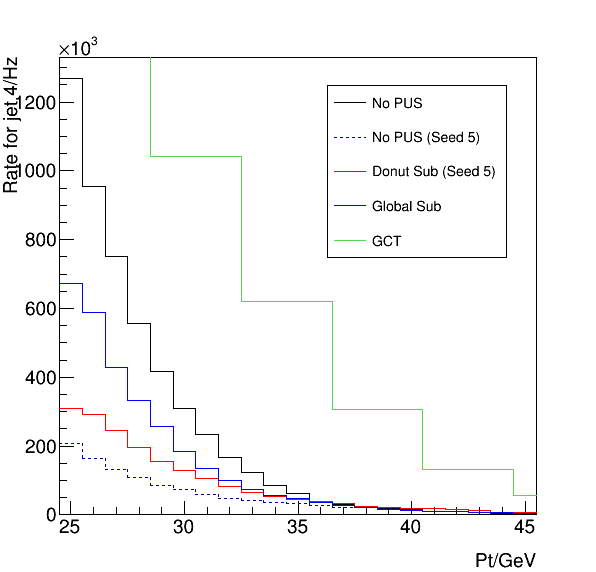
\includegraphics[width=7.2cm]{./Figures/triggerUpgrade/rate3}}
\hfill
\subfigure[Jet 
1 Rate vs Number of Interactions \label{fig:label:ratenvtx}]{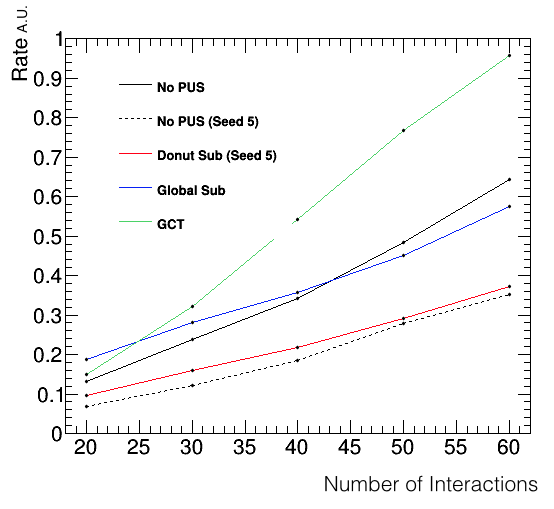
\includegraphics[width=7cm]{./Figures/triggerUpgrade/neutrinonvtx_jet1}}
\caption{In \ref{fig:label:ratejet1} the rate for the 4th jet 
against threshold is shown. This is reduced for stage 2 compared to GCT and for 
pileup subtraction. The dependence of the rate at $p_T=30GeV$ for the lead jet with on 
the number of interactions is shown in figure \ref{fig:label:ratenvtx}}.
\label{fig:label:rates}
\end{figure}
\begin{figure}
\centering
    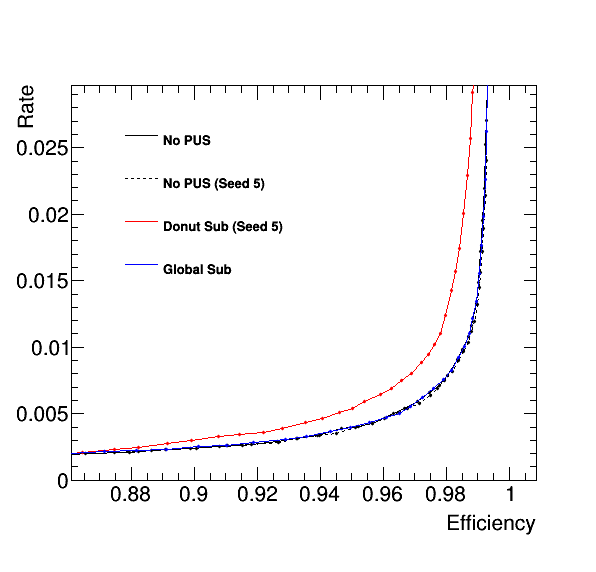
\includegraphics[width=8cm]{././Figures/triggerUpgrade/jet1RateEff}
  \caption{Rate 
  versus efficiency for lead jet. Performance is consistent except for donut which appears to 
  excessively reduce efficiency}
  \label{fig:label:rateeff}
\end{figure}
\subsection{Turn On Plots}
To benchmark the performance of the 
L1 jets their $p_T$ must be compared with matched generator level quantities. To do this 
the generator level quantity is plotted with a cut on the matched L1 quantity (the 
turn on). This is shown in figure \ref{turnon} for the 4th jet. The stage 2 
quantities are shown to be very comparable, however, the   GCT is less sharp and thus 
the agreement with gen worse. 
\begin{figure}
\centering
    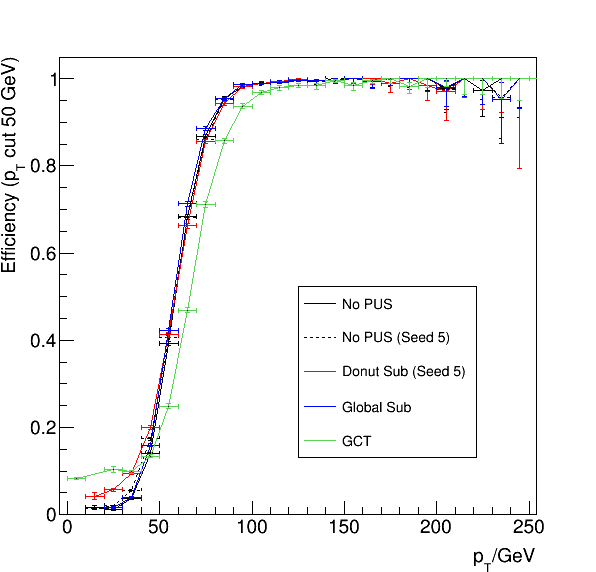
\includegraphics[width=7.5cm]{./Figures/triggerUpgrade/turnon3_50}
  \caption{Turn on curve for the 4th jet 
  at 50 GeV showing comparable behaviour for the stage 2 quantities and a shallower 
  turn on for GCT.}
  \label{turnon}
\end{figure}
\subsection{Energy Sums}
Lastly, the energy sums, \scalht and 
\mht~, were investigated. To nullify the problem of the lower calibration limit, only jets above 
this are included in the sums. This also has the effect of removing the majority 
of remaining clustered pileup jets. Pileup is expected to be approximately uniform and so should 
not affect the missing energy in the event. The results for a $t\bar{t}$ sample are 
shown in figure \ref{fig:label:sums}. Pileup subtraction improves the agreement as compared to gen.  The \scalht 
shows especially good agreement with gen for the case of a seed as compared to 
global $\rho$. This is due to the under subtraction bias of this method. The \mht 
shows similar levels of agreement for all cases as expected. 
\begin{figure}
\hfill
\subfigure[\scalht\label{fig:label:ht}]{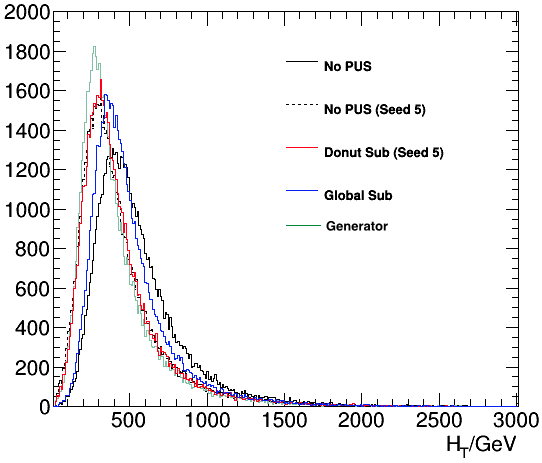
\includegraphics[width=7cm]{./Figures/triggerUpgrade/ht_ttbar}}
\hfill
\subfigure[\mht~\label{fig:label:mht}]{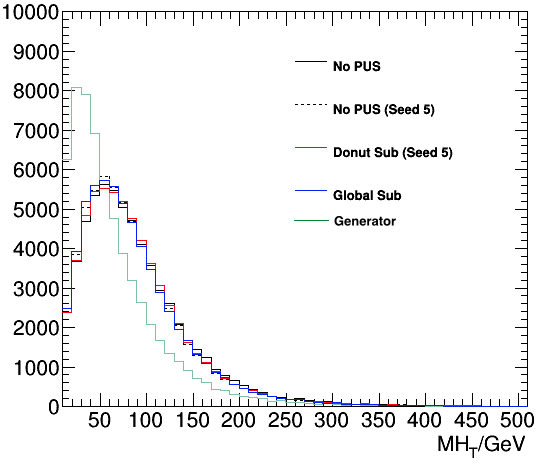
\includegraphics[width=7cm]{./Figures/triggerUpgrade/mht_ttbar}}

\caption{In figure \ref{fig:label:ht} the total energy shows good agreement with the generator level quantity. This 
is improved by requiring a seed threshold. In figure \ref{fig:label:mht} similar agreement is shown for 
all cases}
\label{fig:label:sums}
\end{figure}
\section{Conclusions}
The jet algorithm has been shown to give very compatible 
results with the offline anti-kT algorithm and maintain a high matching efficiency to generator level 
quantities.  Pileup subtraction has been shown to be important for  run 2. While both global 
and donut subtraction have been shown to flatten the response against number of interactions (\ref{fig:label:resolution}) 
each has weaknesses that must be addressed. Figure \ref{fig:label:rateeff} shows that applying a seed threshold 
is comparable to global subtraction at killing rate while maintaining efficiency. Donut subtraction appears to 
perform less well than applying the seed threshold alone. This may be due to the 
susceptibility to fluctuations and contamination. Further studies are underway to increase the sampling area for 
donut subtraction which is expected to improve performance. Figure \ref{fig:label:sums} shows global $\rho$ overestimating the 
$H_T$. This is due to the under-subtraction bias leading to excess energy being left in 
the event. This may be correcting by applying a seed threshold as for donut but 
calculating $\rho$ using all jets. 

Further studies are currently underway to utilise the $\eta$ 
dependence of the pileup in the detector.  The seed threshold applied may be altered depending 
on the location of the tower to further reduce rate in areas of high pileup 
while maintaining efficiency in low pileup regions. Improving calibrations such that lower energy jets may 
be utilised is also key. Finally, increasing the sample size to use $3\times3$ towers for 
the seed should improve discrimination between pileup and boosted jets.
